\documentclass[12pt,letterpaper]{article}
\usepackage[latin1]{inputenc}
\usepackage{amsmath}
\usepackage{amsfonts}
\usepackage{amssymb}

% the above packages are the "base"

\usepackage{graphicx}

\usepackage{hyperref} % enable links within pdf
\hypersetup{colorlinks = true, linkcolor = black, urlcolor = blue}

\usepackage{pdfpages} % enable insertion of another pdf
\usepackage{float} % for [!h] and [H] forcing of figure placement


\setcounter{secnumdepth}{0}  % don't number sections (stars not needed)


\author{}
\title{Getting started with \texttt{Git} \& \texttt{GitHub}}
\date{}

\begin{document}
\maketitle

\tableofcontents

\pagebreak


\section{What is version control?}
Version control software allows you to save and provide meta-information on any and all changes you make to a set of files and directories.
It allows you to more easily document changes and the evolution of your files, find and correct bugs that have crept into your code, and revert back to old versions when needed.
By using version control you'll know what, when and (hopefully) why changes were made.
If you're using the software collaboratively, you'll also know by whom changes were made.
Backing-up is virtually implicit when you also use a networked (off-site) server as a host for your repository.

We'll be using \texttt{Git} as our version control software.
There are others out there (e.g., \texttt{Subversion}).
We'll be using \texttt{GitHub} as our host.
There are others out there (e.g., \texttt{Bitbucket}).

\section{Git}
\texttt{Git} was developed by Linus Torvalds (the ``Linu'' in Linux).
Most of its features are accessed by command-line and are intended for large-scale collaborative programming and software development purposes.
Of course, we'll be using \texttt{Git} for much smaller, specific projects, thus we won't bother with many of these feature.
We'll also interact with \texttt{Git} using GUIs (graphical user interfaces, e.g., \texttt{R-Studio}, \texttt{Sourcetree}) rather than command-line.


\section{GitHub}
\texttt{Git} stores a complete copy of the project on your local machine, including all its history and versions; no centralized server is necessary.
However, if you want to collaborate with others, have multiple computers with which you'd like to work, or want to create true back-ups of your project, then you'll also want to use a server on which to host your repository.
Fortunately, there are a number of free providers.

For \texttt{Git}, the primary options are \texttt{GitHub} and 
\texttt{Bitbucket}.
The former is more developed (more bells and whistles), is currently more widely used, and is perhaps a little easier to work with.
The two don't differ all that much except in one regard:  the number of free versus public repositories.
While \texttt{GitHub} has a limit on the number of private repositories, 
\texttt{Bitbucket} has a limit on the number of collaborative projects (having 
more than 5 collaborators).
(There are perks regarding the number of repositories you can have if you sign up using an academic email address.  See \url{https://help.github.com/en/articles/applying-for-an-educator-or-researcher-discount})



\section{Installing and configuring Git}
See the \texttt{README.md} of our very first class for installing \texttt{Git}.

After installation, there's a little (minimum of) command-line configuration to perform.
On a Mac, open a \texttt{Terminal} window and type in the following:

\noindent
     \texttt{\$ git config --global user.name "Mark Novak"}\\
     \texttt{\$ git config --global user.email "Mark.Novak@oregonstate.edu"}

\noindent
Some of you might want to set up an editor to be used in git, for example:

\noindent
	\texttt{\$ git config --global core.editor atom}

\noindent
(replacing \texttt{atom} for the name of your editor).
You can check to ensure that these commands went through and see what other things you might want to configure using

\noindent
\texttt{\$ git config --list}

\noindent
For more, or if you're using Windows, see\\
\begin{footnotesize}
\url{https://git-scm.com/book/en/v2/Getting-Started-First-Time-Git-Setup}
\end{footnotesize}




\section{Repository setup}
There are command-line methods for doing everything we're going to do below.
Indeed, command-line is the default way to interact with \texttt{Git}.\footnote{See last page for a cheat sheet.}
Instead, we're mostly going to make use of the tools made available through 
\texttt{GitHub}, starting with the very first step of initiating a repository and 
getting some minimal information associated with it.
That is, rather than creating and setting up a repository on our computer by 
command-line and then connecting it to \texttt{GitHub}, we'll create and set up 
the repository on \texttt{GitHub} and then clone it to our local master folder of 
projects.

Simply login to your \texttt{GitHub} account, click on ``New Repository'', and 
follow the instructions.\footnote{When doing so, be sure you're in your own user 
environment and not inside our Analytical Workflows organization.}
These should include options for private vs. public (the latter is preferred for this class\footnote{If at all possible, please pick public (for this class) and switch to private afterwards.  Otherwise, please add me as a collaborator so I can see your repo.}), initializing with a \texttt{README.md} file (which you \emph{should} do), and adding a \texttt{.gitignore} file (which you \emph{should} also do).

The \texttt{README.md} file in the main repo folder is the first file that anyone will see when they inspect your repository (assuming it's public).
At minimum, it should give an overview of what the project is about and what the various parts of the project structure are.
We will learn to use Markdown to write and edit \texttt{README.md} files later in the course, so for now just leave it as is.

The \texttt{.gitignore} file contains a list of all the files that you want \texttt{Git} to ignore (i.e. not monitor for changes).
Selecting \texttt{R} from the dropdown list will auto-populate a bunch of it for you.
Later in the course, we'll also add the extensions for all the temporary files that \LaTeX\ produces when compiling.

You should now see a new webpage -- your Repo page -- that shows you what's in your repository.
For now it contains only the \texttt{.gitignore} and \texttt{README.md} files, the 
latter of which has its contents displayed.\footnote{There are actually other files 
in your folder as well, but they're hidden by default.}
As I said earlier, there are a lot of bells-and-whistles at your fingertips here.
We'll ignore them for now, but feel free to explore!
You \emph{could} start dragging-in directories and files into your browswer view to add them to your repository, but we're \emph{not} going to do that.
Instead, we're going to \texttt{clone} this repository to our local machine, then add our various project sub-folders to it (e.g., \texttt{code}, \texttt{data}, and \texttt{results}), and go from there.\footnote{Note that empty folders will not be monitored by \texttt{Git}; they need to contain something.}

To clone the repository, click the green \texttt{Clone or download} button and copy the provided URL.
There's a few ways to clone your repository to your local machine.
Your preferred method depends on how you're likely to interface with \texttt{Git}.
You could:
\begin{enumerate}
	\item use command-line to clone.  Open \texttt{Terminal}, \texttt{cd} into your \texttt{Projects} master folder, then type \texttt{git clone} followed by the URL you just copied;
	\item use a visual \texttt{Git} GUI client to clone the repo;
\end{enumerate}
or, if you're primarily going to be using this repository to keep track of an \texttt{R}-based project using \texttt{R-Studio}:
\begin{enumerate}
  \setcounter{enumi}{2}
	\item set up a ``project'' within \texttt{R-Studio} first and provide it with the URL during setup.  It'll then clone the repo for you.
\end{enumerate}

\section{R-Studio and Git GUIs}
I use \texttt{Git} for both \texttt{R} and non-\texttt{R} (e.g.,  \texttt{Mathematica})-based projects.
Only  \texttt{R-Studio} has integrated  \texttt{Git} functionality, so I use a visual  \texttt{Git} GUI client (e.g., \texttt{Sourcetree}) for some projects because I haven't yet bothered to memorize the  \texttt{Git} command-line commands.
Since most of you are probably using \texttt{R}, it's probably worthwhile to start 
off by using \texttt{R-Studio}'s \texttt{Git} integration feature.
(Note, however, that \texttt{R-Studio} isn't able to do useful things, like 
branching, which we'll cover later.  Therefore you'll still benefit from using a 
\texttt{Git} GUI or learning the commands.)

You'll first need to tell \texttt{R-Studio} that you have \texttt{Git} installed, so go to its Preferences, select \texttt{Git/SVN} and fill in the details: either click on the Help link or go to
\url{http://r-pkgs.had.co.nz/git.html} to see what to do.

Now create your ``project'' within  \texttt{R-Studio} by selecting ``New Project''.
Select \texttt{Version Control: Checkout a project from...repository}, select 
\texttt{Git}, and fill in the details including the URL you got from \texttt{GitHub}.
The directory in which you place your repository should be your master folder.
\texttt{R-Studio} will ``restart'' and then you'll be in your project (as evidenced by its name appearing in the top-right of the interface).
Clicking on the \texttt{Files} tab will show you what's in the repository (which should, at present, be: \texttt{README.md}, \texttt{.gitignore} and the newly created \texttt{.Rproj} file).

You may now create (or move in) all your project sub-folders.




\section{Git workflow}
Before proceeding, jump over and do the \textbf{required reading:}\\
\url{https://git-scm.com/book/en/v2/Getting-Started-What-is-Git%3F}.\\
Then come back here.

Basically, files (or directories) exist in one of four states of a life-cycle: \emph{untracked}, \emph{staged}, \emph{unmodified}, or \emph{modified} (see Fig. \ref{fig:lifecycle}).
The standard workflow is thus:
\begin{enumerate}
	\item Add or modify some files;
	\item Stage the new or modified files;
	\item Commit the changed files (moving them from the Staging Area to the 
	``memory'' of the repository);
	\item Repeat.
\end{enumerate}

\begin{figure}
	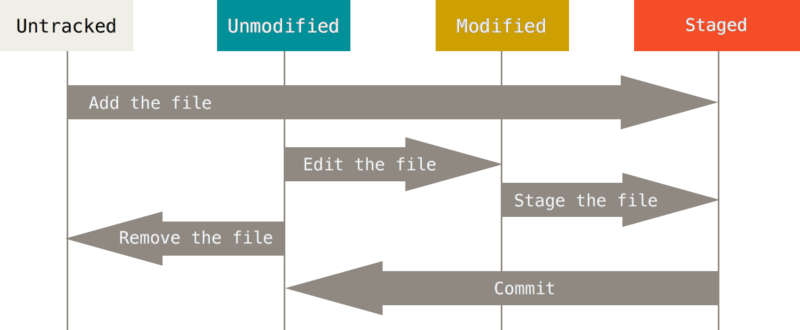
\includegraphics[width=\linewidth]{figs/lifecycle}
	\caption{The \texttt{Git} life-cycle.}
	\label{fig:lifecycle}
\end{figure}

Your motto for using \texttt{Git} should be ``\emph{commit early, commit often}''.
Almost every time you add or remove something from your project (i.e. a file or 
a chunk of code), you want to commit those changes.
Ideally, each commit should correspond to a ``logical unit'', one that you are able to describe in a few words (e.g., ``Add function to perform resampling'').
Choosing when to commit is quite important, especially when you're debugging code.
For example, if you've discovered your code has two bugs, then you should 
commit each one of the fixes seperately, not together.
That way you can undo either fix independently if, for example, you messed up in one of your fixes or your fix created a different bug somewhere else in your code.\footnote{We'll talk about using ``branches'' to reduce the incidence of problems down the road.}

\texttt{Git} GUIs provide visual interfaces for viewing your files, staging area, 
and commits.
Within \texttt{R-Studio} (assuming you have your \texttt{R-Studio} project 
opened), looking at the \texttt{Git} tab will show you a list of all the files (and 
directories) that have been changed, removed, or added to the project since the 
last time you committed.
Clicking on the check-boxes associated with each file will add them to the staging area.
Clicking on \texttt{Diff} or \texttt{Commit} will open up a new interface (the staging area).
In the top-left corner you'll see a list of the staged files.
Selecting one of the files will bring its contents up in the window below which highlights the text that has been added (in green) and removed (in red).
Select all the files you want to commit, stage them, add a commit message to the top-right window, and commit.
You've now updated your local respository.
Clicking on \texttt{History} (top-left) will show you all your past commits.

How to write good commit messages is a topic unto itself!  
For now, the only things we'll say are 
\begin{enumerate}
	\item that a properly-formed \texttt{Git} commit subject line should always 
	complete the following sentence:  
``If applied, this commit will \emph{your subject line here...}''\footnote{Every 
commit 
message must at minimum have a ``subject line''.  
In fact, the subject line could be the only thing in your message.  
However, you can also write a whole lot more if you'd like, a paragraph even, 
by adding a blank second line between the subject line and the rest of your 
message.  
For a great post on writing commit messages, see 
\url{https://chris.beams.io/posts/git-commit/}.};
	\item capitalize the first word; and
	\item don't use a period at the end of the sentence.	
\end{enumerate} 

\textbf{Remember, ``\emph{commit early, commit often}'' and provided concise 
and informative commit messages (Fig.~\ref{fig:commit_messages}).}

The final thing to do (not necessarily following each commit) is to \texttt{Push} 
your commit to \texttt{GitHub}.
\texttt{Pull} does the opposite: bringing commits that have been saved to 
\texttt{GitHub} (by others, or by you on a different machine) to your local 
machine.
To reduce the likelihood of creating conflicts, \emph{always} pull before you start making edits, commit and push.
There are of course ways of dealing with conflicts and merging files (that will arise if collaborator(s) are working on the same file, for example), but pulling first will do a lot to avoid unneccessary hassle.\footnote{We'll learn about merging and conflict resolution later in the course.}

\
So again, our basic recipe is:
\begin{center}
	\textbf{\emph{pull, create/edit, stage,commit, push, repeat.}}
\end{center}

\begin{figure}[!h]
	\centering
	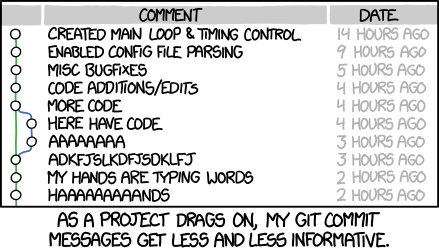
\includegraphics[width=0.7\linewidth]{figs/xkcd_git_commit}
	\caption{Don't let this happen!  (source: \url{http://xkcd.com/1296/})}
	\label{fig:commit_messages}
\end{figure}

\clearpage

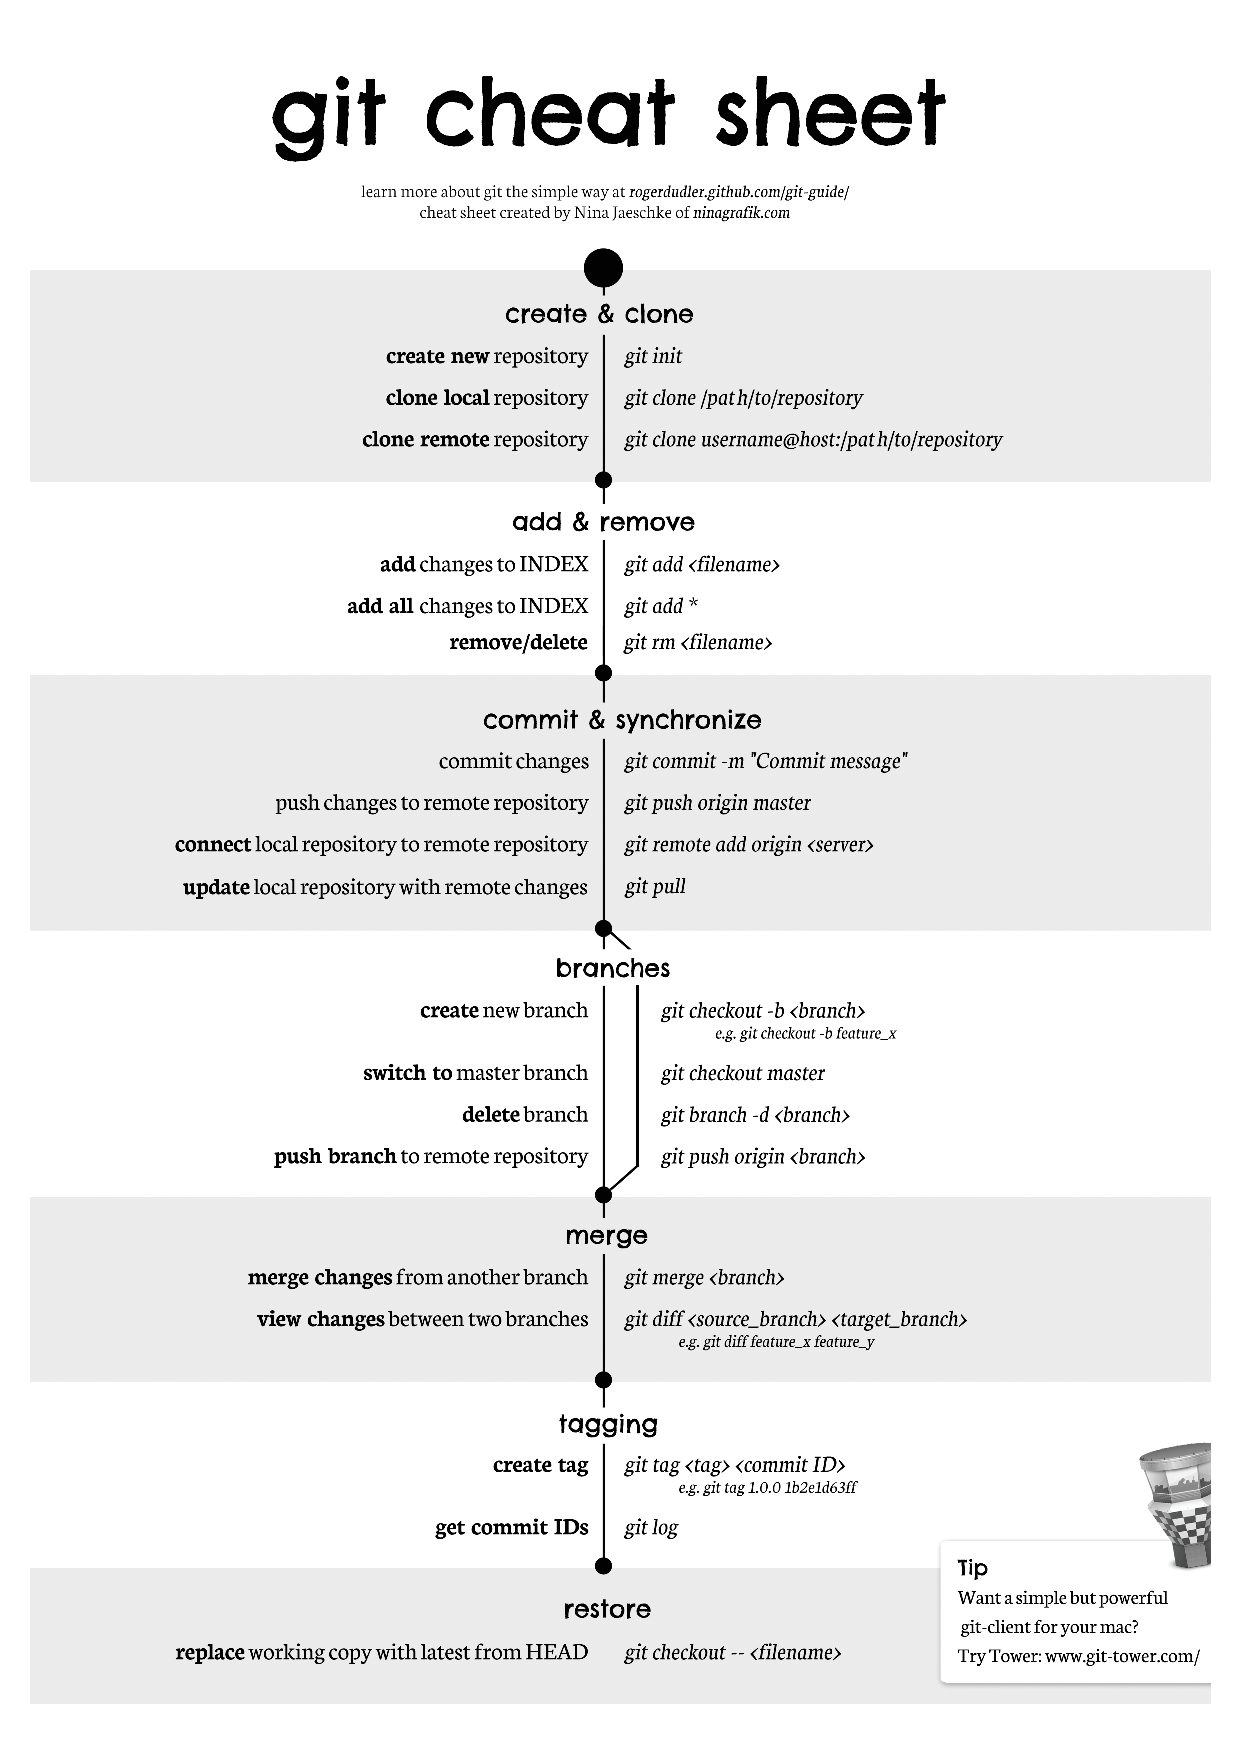
\includepdf{../reference/git_cheat_sheet.pdf}

\end{document}
